\begin{figure}
	
	\begin{center}	
		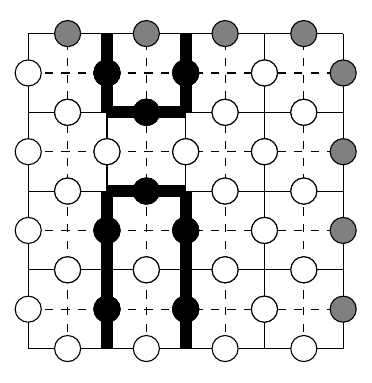
\begin{tikzpicture}
			% Draw dashed lines
			\foreach \i in {-2,-1.5,...,2}
			{
				\draw[dashed] (\i,-2) -- (\i,2);
			}
			\foreach \j in {-2,-1.5,...,2}
			{
				\draw[dashed] (-2,\j) -- (2,\j);
			}
			
			% Draw solid grid and nodes with circles in the middle of each side
			\draw[step=1cm] (-2,-2) grid (2,2);
			\foreach \i in {-1.5,...,1.5}
			{
				\foreach \j in {-1.5,...,1.5}
				{
					\begin{scope}[transform canvas={xshift=\i cm,yshift=\j cm}]
						\node[right,xshift=0.2cm,yshift=0.4cm] {};
						% Convert \j and \i to integers
						\pgfmathtruncatemacro{\intj}{\j}
						\pgfmathtruncatemacro{\inti}{\i}
						
						% Draw circles at the midpoints of each side
						\ifnum\intj=1
						\draw node[draw,circle,fill=gray] at (0,0.5) {};
						\else
						\draw node[draw,circle,fill=white] at (0,0.5) {};
						\fi
						
						\ifnum\inti=1
						\draw node[draw,circle,fill=gray] at (0.5,0) {};
						\else
						\draw node[draw,circle,fill=white] at (0.5,0) {};
						\fi
						
						\draw node[draw,circle,fill=white] at (0,-0.5) {};
						\draw node[draw,circle,fill=white] at (-0.5,0) {};
					\end{scope}
				}
			}
			
			\foreach \i in {0,...,0}
			{
				\draw[black, line width=1.5mm] (\i,-2) -- (\i,0);
				\draw[black, line width=1.5mm] (\i,1) -- (\i,2);
				\node[draw, circle, fill=black] at (\i,-0.5) {};
				
				\node[draw, circle, fill=black] at (\i,-1.5) {};
				\node[draw, circle, fill=black] at (\i,1.5) {};		
				
			}
			
			\foreach \i in {-1,...,-1}
			{
				\draw[black, line width=1.5mm] (\i,-2) -- (\i,0);
				\draw[black, line width=1.5mm] (\i,1) -- (\i,2);
				\node[draw, circle, fill=black] at (\i,-0.5) {};
				
				\node[draw, circle, fill=black] at (\i,-1.5) {};
				\node[draw, circle, fill=black] at (\i,1.5) {};		
				
			}
			
			\foreach \i in {-1,...,-1}
			{
				
				\draw[black, line width=1.5mm] (\i,1) -- (\i,2);
				\node[draw, circle, fill=black] at (\i,1.5) {};
				
			}
			
			\foreach \j in {0,...,0}
			{
				\draw[black, line width=1.5mm] (-1,\j) -- (0,\j);
				\node[draw, circle, fill=black] at (-0.5,\j) {};		
				
			}
			
			\foreach \j in {1,...,1}
			{
				\draw[black, line width=1.5mm] (-1,\j) -- (0,\j);
				\node[draw, circle, fill=black] at (-0.5,\j) {};
				\node[draw, circle, black] at (-0.5,\j) {};	
				
			}
			
			
		\end{tikzpicture}	
		
		\vspace{1cm} 
		
		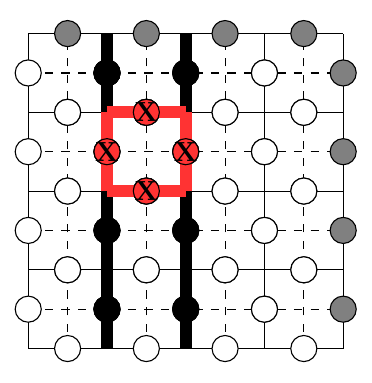
\begin{tikzpicture}
			% Draw dashed lines
			\foreach \i in {-2,-1.5,...,2}
			{
				\draw[dashed] (\i,-2) -- (\i,2);
			}
			\foreach \j in {-2,-1.5,...,2}
			{
				\draw[dashed] (-2,\j) -- (2,\j);
			}
			
			% Draw solid grid and nodes with circles in the middle of each side
			\draw[step=1cm] (-2,-2) grid (2,2);
			\foreach \i in {-1.5,...,1.5}
			{
				\foreach \j in {-1.5,...,1.5}
				{
					\begin{scope}[transform canvas={xshift=\i cm,yshift=\j cm}]
						\node[right,xshift=0.2cm,yshift=0.4cm] {};
						% Convert \j and \i to integers
						\pgfmathtruncatemacro{\intj}{\j}
						\pgfmathtruncatemacro{\inti}{\i}
						
						% Draw circles at the midpoints of each side
						\ifnum\intj=1
						\draw node[draw,circle,fill=gray] at (0,0.5) {};
						\else
						\draw node[draw,circle,fill=white] at (0,0.5) {};
						\fi
						
						\ifnum\inti=1
						\draw node[draw,circle,fill=gray] at (0.5,0) {};
						\else
						\draw node[draw,circle,fill=white] at (0.5,0) {};
						\fi
						
						\draw node[draw,circle,fill=white] at (0,-0.5) {};
						\draw node[draw,circle,fill=white] at (-0.5,0) {};
					\end{scope}
				}
			}
			
			\foreach \i in {0,...,0}
			{
				\draw[black, line width=1.5mm] (\i,-2) -- (\i,0);
				\draw[black, line width=1.5mm] (\i,1) -- (\i,2);
				\node[draw, circle, fill=black] at (\i,-0.5) {};
				
				\node[draw, circle, fill=black] at (\i,-1.5) {};
				\node[draw, circle, fill=black] at (\i,1.5) {};		
				
				\draw[red!80, line width=1.5mm] (\i,0) -- (\i,1);
				\node[draw, circle, fill=red!80, label = center:\textbf{X}] at (\i,0.5) {};		
				
			}
			
			\foreach \i in {-1,...,-1}
			{
				\draw[black, line width=1.5mm] (\i,-2) -- (\i,0);
				\draw[black, line width=1.5mm] (\i,1) -- (\i,2);
				\node[draw, circle, fill=black] at (\i,-0.5) {};
				
				\node[draw, circle, fill=black] at (\i,-1.5) {};
				\node[draw, circle, fill=black] at (\i,1.5) {};		
				
				
				
			}
			
			\foreach \i in {-1,...,-1}
			{
				
				\draw[black, line width=1.5mm] (\i,1) -- (\i,2);
				\draw[red!80, line width=1.5mm] (\i,0) -- (\i,1);
				\node[draw, circle, fill=black] at (\i,1.5) {};
				\node[draw, circle, fill=red!80,label = center:\textbf{X}] at (\i,0.5) {};
				
			}
			
			\foreach \j in {0,...,0}
			{
				\draw[red!80, line width=1.5mm] (-1,\j) -- (0,\j);
				\node[draw, circle, fill=red!80,label = center:\textbf{X}] at (-0.5,\j) {};		
				
			}
			
			\foreach \j in {1,...,1}
			{
				\draw[red!80, line width=1.5mm] (-1,\j) -- (0,\j);
				\node[draw, circle, fill=red!80,label = center:\textbf{X}] at (-0.5,\j) {};
				
				
			}
			
			
		\end{tikzpicture}	
		
		\vspace{1cm} 
		
		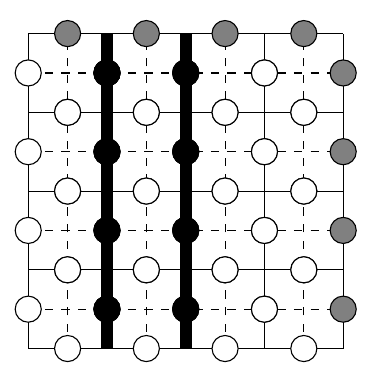
\begin{tikzpicture}
			% Draw dashed lines
			\foreach \i in {-2,-1.5,...,2}
			{
				\draw[dashed] (\i,-2) -- (\i,2);
			}
			\foreach \j in {-2,-1.5,...,2}
			{
				\draw[dashed] (-2,\j) -- (2,\j);
			}
			
			% Draw solid grid and nodes with circles in the middle of each side
			\draw[step=1cm] (-2,-2) grid (2,2);
			\foreach \i in {-1.5,...,1.5}
			{
				\foreach \j in {-1.5,...,1.5}
				{
					\begin{scope}[transform canvas={xshift=\i cm,yshift=\j cm}]
						\node[right,xshift=0.2cm,yshift=0.4cm] {};
						% Convert \j and \i to integers
						\pgfmathtruncatemacro{\intj}{\j}
						\pgfmathtruncatemacro{\inti}{\i}
						
						% Draw circles at the midpoints of each side
						\ifnum\intj=1
						\draw node[draw,circle,fill=gray] at (0,0.5) {};
						\else
						\draw node[draw,circle,fill=white] at (0,0.5) {};
						\fi
						
						\ifnum\inti=1
						\draw node[draw,circle,fill=gray] at (0.5,0) {};
						\else
						\draw node[draw,circle,fill=white] at (0.5,0) {};
						\fi
						
						\draw node[draw,circle,fill=white] at (0,-0.5) {};
						\draw node[draw,circle,fill=white] at (-0.5,0) {};
					\end{scope}
				}
			}
			
			\foreach \i in {0,...,0}
			{
				\draw[black, line width=1.5mm] (\i,-2) -- (\i,0);
				\draw[black, line width=1.5mm] (\i,1) -- (\i,2);
				\node[draw, circle, fill=black] at (\i,-0.5) {};
				
				\node[draw, circle, fill=black] at (\i,-1.5) {};
				\node[draw, circle, fill=black] at (\i,1.5) {};		
				
				\draw[black, line width=1.5mm] (\i,0) -- (\i,1);
				\node[draw, circle, fill=black] at (\i,0.5) {};		
				
			}
			
			\foreach \i in {-1,...,-1}
			{
				\draw[black, line width=1.5mm] (\i,-2) -- (\i,0);
				\draw[black, line width=1.5mm] (\i,1) -- (\i,2);
				\node[draw, circle, fill=black] at (\i,-0.5) {};
				
				\node[draw, circle, fill=black] at (\i,-1.5) {};
				\node[draw, circle, fill=black] at (\i,1.5) {};		
				
				
				
			}
			
			\foreach \i in {-1,...,-1}
			{
				
				\draw[black, line width=1.5mm] (\i,1) -- (\i,2);
				\draw[black, line width=1.5mm] (\i,0) -- (\i,1);
				\node[draw, circle, fill=black] at (\i,1.5) {};
				\node[draw, circle, fill=black] at (\i,0.5) {};
				
			}
			
			
			
		\end{tikzpicture}	
		

	\end{center}

\caption{Apply $Bp$ to a closed loop.}
\label{fig:Bpstrano}
\end{figure}
